% Metódy inžinierskej práce

\documentclass[10pt,twoside,slovak,a4paper]{article}

\usepackage[slovak]{babel}
%\usepackage[T1]{fontenc}
\usepackage[IL2]{fontenc} % lepšia sadzba písmena Ľ než v T1
\usepackage[utf8]{inputenc}
\usepackage{graphicx}
\usepackage{url} % príkaz \url na formátovanie URL
\usepackage{hyperref} % odkazy v texte budú aktívne (pri niektorých triedach dokumentov spôsobuje posun textu)

\usepackage{cite}
%\usepackage{times}



\title{Herné umenie\thanks{Semestrálny projekt v predmete Metódy inžinierskej práce, ak. rok 2022/23, vedenie: Meno Priezvisko}} % meno a priezvisko vyučujúceho na cvičeniach

\author{Marek Fiľo\\[2pt]
	{\small Slovenská technická univerzita v Bratislave}\\
	{\small Fakulta informatiky a informačných technológií}\\
	{\small \texttt{xfilo@stuba.sk}}
	}

\date{\small 30. september 2022} % upravte



\begin{document}

\maketitle

\begin{abstract}


Cieľom tohto článku je priblížiť čitateľovi pojemy \emph{Herné umenie}, \emph{Herný umelec} a pribížiť časti, na ktoré sa delí. Pozrieme sa aj na to ako herné umenie ovplyvňuje popularitu hry a či je to hlavný faktor, ktorý ovplyvňuje úspešnosť hry.
\end{abstract}




\section{Úvod} \label{začiatok}
Vznik herného umenia ako ho poznáme dnes podmienil vznik počítačov a ich rozšírenie medzi širokú verejnosť.
Pod slovným spojením  \emph{Herné umenie} si môže niekto predstaviť perfektne zahranú hru či už šachu alebo niektorej z moderných počítačových hier. My pod týmto názvom rozumieme vizuálne prevedenie hry. Všetko čo vidíme na obrazovke alebo aj na našom stole je výsledkom práce herných umelcov, ktorých úlohou bolo vytvoriť návrhy a výsledné prevedenia toho čo vidíme, tak aby to odpovadalo téme hry, časovému obdobiu v ktorom sa hra odohráva a taktiež žánru hry.














\section{Herný umelec} \label{pokračovanie}
Herný umelec je človek, ktorý ma na svedomí vzhľad prostredia, postáv a všetkých ostatných prvkov, ktoré sa v hre vyskytujú. Umelcov rozdeľujeme na nasledovné kategórie.
\paragraph{Koncepčný umelec} Dáva základnú podobu v 2D všetkému čo sa v hre vyskytuje. S jeho návrhmi pracujú ostatný umelci a dávajú im finálnu podobu.

\paragraph{Umelec prostredia} Vytvára prostredie, modeluje 3D modely prvkov, ktoré sa v ňom nachádzajú napr. strom, dom.

\paragraph{Charakterový umelec} Výtvára vzhľad postáv.
\paragraph{Animátor postáv} Špeciálny typ 3D animátora, ktorý vdychuje život postavám.
\paragraph{FX animátor}Je zodpovedný za všetky špeciálne efekty ako napríklad výbuchy, oheň a mnohé iné. Jeho úlohou je aby tieto efekty vyzerali reálne a divák si nemyslel že sú počítačivo generované.

\section{Ako sa stať herným umelcom}
Herné umenie ako každé iné si vyžaduje kreativitu a kúsok talentu. Najprv sa treba zamerať na základy ako sú kreslenie, perspektíva, tieňovanie a hĺbka. Neodmysliteľnou súčasťou je práve kreslenie, treba sa v ňom zlepšovať a cvičiť najlepšie každý deň. Ďalším krokom je práca s programami na tvorbu grafiky, prit výbere programu, v ktorom budete pracovať záleží na tom či chcete tvoriť 2D alebo 3D grafiku. Jeden z najznámejších porgramov pre 2D grafiku je Adobe Photoshop, pre 3D grafiku to je Maya a 3DS Max, ktoré sú používané mnohými spoločnosťami.
\cite{1}
\section{Ukážka grafických programov}





\section{2D štýly herného umenia}
\cite{2D}
\paragraph{Pixel art}
Jeden z najpopulárnejších štýlov 2D. Mnoho ľudí si Pixel art spája s prvými videohrami ale tento šlýl má slušné zastúpenie aj v tejto dobe. 
To the Moon


\paragraph{Vector art}
Ako už z názvu vyplýva v tomto štýle sa pracuje s vektorovými obrázkami. Obrázky sa nerozdeľujú na jednotlivé pixely ale ukladá ich pomocou geometrických tvarov. Výhodou je menšia veľkosť obrázkov a jedinečný vzhľad hry.

\paragraph{Cutout art}
Ako už meno napovedá, tento štýl napodobňuje obrázky nakreslené na papieri a vložené do hry. Obraz výrezu ostáva nemenný, mení sa jeho poloha aby simulovala akcia alebo obraz výrezu môže byť nahradený iným výrezon na simuláciu zmeny stavu.
Don't Starve

\paragraph{Cel Shading art}
Tento štýl sa snaží vytvoriť 3D modely a objekty tak, aby vyzerali ako 2D
Borderlands
\paragraph{Monochromatic art}
Vyznačuje sa veľmi limitovanou paletou farieb, zväčša 1 alebo 2 farby. A však v hre je použitých mnoho odtieňov pre lepšie rozlišovanie medzi objektami.
Limbo
\paragraph{Flat art}
Postavy v hre sú bez hĺbky a objemu. Nenájdeme tu žiadne reálne prvky a ani prvky fyziky. V tomto štýle majú umelci takmer úplnú voľnosť.
Flat Kingdom
\paragraph{Doodle art}
Tento štýl je definovaný hlavne svojím osobitým vzhľadom. Postavy a prvky prostredia majú netradičný vzhľad a často sú zložené z viacerých samostatných prvkov.
Doodle jump


\section{3D štýly herného umenia}

\paragraph{Realizmus}
Zámerom je vytvoriť grafiku, ktorá vyzerá čo najvia podobá na realitu. Najväčšie AAA tituly vychádzajú v tomto štýle. Časová línia môže byť zasadená do ktorého koľvek obdobia, dej a žáner hry sa s realitou nemusia vôbec podobať.
Phasmophobia

\paragraph{Fantasy realizmus}
Tento štýl sa od predchádzajúceho odlišuje najmä v žánre hier, v ktorých sa vyskytuje. Grafika sa podobá realite ale príbeh a dej nemá s realitou nič spoločné. Hráčovi vie priniesť maximálny herný zážitok spolu s umelckou hodnotou.
God of War

\paragraph{Low Poly}
Podstatou tohto štýlu je zobrazovanie objektov pomocou mnohouholníkov. Každý má jednu farbu, ktorá sa nemení. Z názvu by sa dalo usúdiť že sa jedná o štýl s malou kvalitou obrazu ale nie je to tak, v jednej hre sa môže vyskytovať okolo milióna jednotlivých tvarov.
Poly Bridge

\paragraph{}
\begin{figure}
\begin{center}
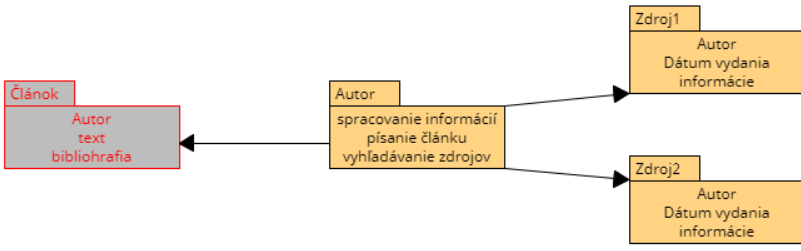
\includegraphics[width=12cm]{diagram novy.png}
\caption{Diagram}
\end{center}
\end{figure}

























%\acknowledgement{Ak niekomu chcete poďakovať\ldots}


% týmto sa generuje zoznam literatúry z obsahu súboru literatura.bib podľa toho, na čo sa v článku odkazujete
\bibliography{literatura}
\bibliographystyle{abbrv} % pabbrvrípadne alpha, abbrv alebo hociktorý iný
\end{document}
